%! Licence = CC BY-NC-SA 4.0

%! Author = gianfluetsch
%! Date = 22. Jan 2022
%! Project = icth_summary

\section{Abtastung von BPSK-Signalen}

\subsubsection{A}
Ein zufälliges bipolares NRZ Datensignal d(t) mit einer Datenrate von 2 Mbit/s wird mit Binary Phase Shift Keying (BPSK) auf eineTrägerfrequenz $f_0 = 5 MHz$ aufmoduliert:\\
$s(t)=d(t)cos(2\pi f_0t)$\\

Das modulierte Trägersignal s(t) hat folgendes zweiseitiges Dichtespektrum S(f):\\
\begin{center}
    \vspace{-8pt}
    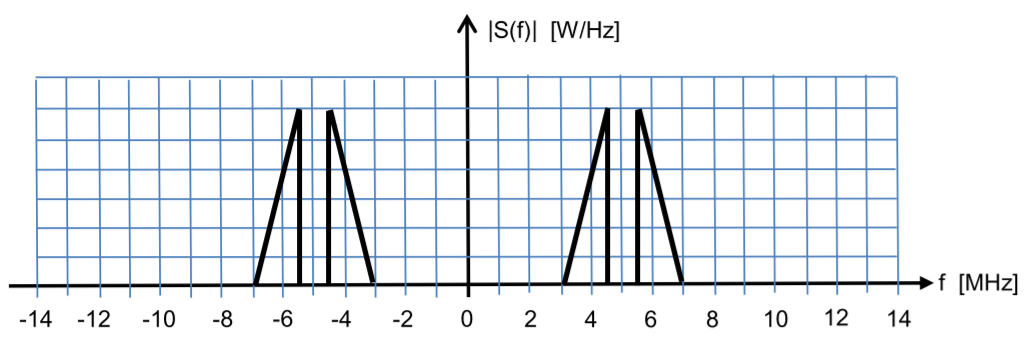
\includegraphics[width=.8\linewidth]{./08-einzelpulse/hs2019_2}
    \vspace{-8pt}
\end{center}

Dieses Trägersignal s(t) wird nun mit einer Samplingfrequenz $f_s = 5 MHz$ abgetastet. Zeichnen Sie das resultierende zweiseitige Spektrum des abgetasteten Signals in die
untenstehende Grafik ein:
\begin{center}
    \vspace{-8pt}
    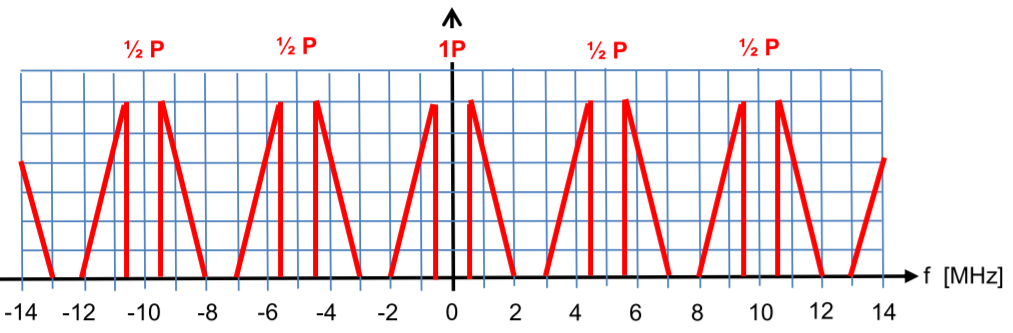
\includegraphics[width=.8\linewidth]{./08-einzelpulse/hs2019_3}
    \vspace{-8pt}
\end{center}

\textbf{Tritt bei dieser Abtastung Aliasing auf?}\\
Hier überlappen sich die Spektrumswiederholungen nicht.\\
So können diese wieder herausgefiltert werden.\\
$\rightarrow$ Es tritt kein Aliasing auf!\\

\textbf{Was bewirkt die gezielte Wahl der Sampling Frequenz $f_s = f_0$?}\\
Sampling mit $f_0$ bewirkt die Verschiebung des Datensignals in das BAsisband und damit eine Produktemodulation.\\

In der folgenden Grafik ist das BPSK-modulierte Trägersignal s(t) dargestellt. Tragen Sie darin die Abtastwerte s[n] ein, die wie folgt definiert sind:\\
$s[n]=s(n*\Delta t)$ mit $\Delta t = \frac{1}{f_s}$
\begin{center}
    \vspace{-8pt}
    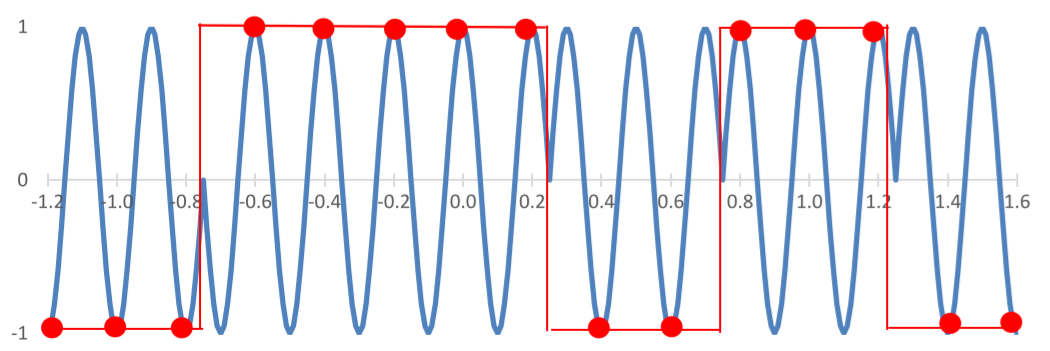
\includegraphics[width=.8\linewidth]{./09-bpsk/hs2019_4}
    \vspace{-8pt}
\end{center}

\textbf{Was stellt das zeitkontinuierliche Signal dar, welches durch Interpolation aus den Abtastwerten s[n] rekonstruiert werden kann?}\\
Das rekonstruierte Signal stellt angenähert das bipolare NRZ Datensignal d(t) dar.\\

\textbf{Welche Datenbits werden durch den obenstehenden Ausschnitt der BPSK Modulation übertragen, unter der Annahme, dass $0°$ Phase eine logische Eins und $180°$ eine logische
Null codiert?}\\
Die Datenfolge lautet: 0 1 1 0 1 0

\subsubsection{B}

In der folgenden Grafik ist das BPSK-modulierte Trägersignal s(t) dargestellt. Tragen Sie darin die Abtastwerte s[n] ein, die wie folgt definiert sind:\\
$s[n]=s(n*\Delta t)$ mit $\Delta t=\frac{1}{f_s}$
\begin{center}
    \vspace{-8pt}
    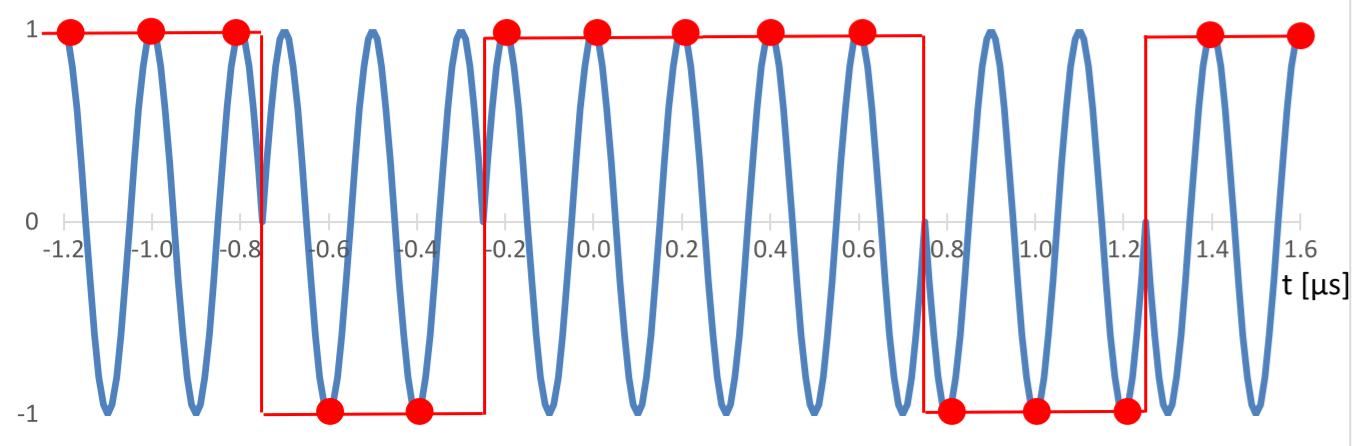
\includegraphics[width=.8\linewidth]{./09-bpsk/hs2018_3}
    \vspace{-8pt}
\end{center}

\textbf{Was stellt das zeitkontinuierliche Signal dar, welches durch Interpolation aus den Abtastwerten s[n] rekonstruiert werden kann?}\\
Das rekonstruierte Signal stellt angenähert das bipolare NRZ Datensignal d(t) dar.\\

\textbf{Welche Datenbits werden durch den obenstehenden Ausschnitt der BPSK Modulation übertragen, unter der Annahme, dass 0° Phase eine logische Eins und 180° eine logische
Null codiert?}\\
$cos(0)=1 \rightarrow 1$\\
$cos(180)=-1 \rightarrow 0$\\
\textit{$\rightarrow$ 1 0 1 1 0 1}


